\subsection{Lab20:Modulacion digital QAM}

%*********************
\begin{frame}{}

\pgfdeclareimage[width=\paperwidth,height=\paperheight]{bg}{imagenes/fondo_lab}
\setbeamertemplate{background}{\pgfuseimage{bg}}

\bfseries{\textrm{\LARGE Lab20\\ \Large Modulacion QAM}}
\raggedright
\end{frame}
%*********************

\begin{frame}{Modulacion de amplitud en cuadratura QAM}
\begin{flushleft}
La modulación de amplitud en cuadratura, en inglés Quadrature Amplitude Modulation (QAM), es una técnica de modulación digital avanzada que transporta datos, técnica en la cual la informacion va a ser modulada tanto en amplitud como en fase (la señal de portadora va a ser modificada en amplitud y fase) o sea que la informacion digital está contenida, tanto en la amplitud como en la fase de la portadora trasmitida. Esto se consigue modulando una misma portadora, desfasando 90º la fase y la amplitud.
\end{flushleft}

La modulación QAM, es una forma de modulación digital en donde la información digital está contenida, tanto en la amplitud como en la fase de la portadora trasmitida.
\end{frame}
%*********************

\begin{frame}{Modulacion de amplitud en cuadratura QAM}
La modulación QAM consiste en modular por desplazamiento en amplitud (ASK) de forma independiente, dos señales portadoras que tienen la misma frecuencia pero que están desfasadas entre sí 90º. La señal modulada QAM es el resultado de sumar ambas señales ASK. Estas pueden operar por el mismo canal sin interferencia mutua porque sus portadoras están en cuadratura. La ecuación matemática de una señal modulada en QAM es:


se encarga de entregar un numero en bits para que el modulador genere la señal en if
${ a }_{ n }\cos { (wt) } +b_{ n }\sin { wt } $
 

\begin{figure}[H]
\centering
\includegraphics[width=.8\textwidth]{Modulaciones_digitales/lab20/pdf/lab20_1.pdf}
\end{figure}
\end{frame}
%*********************

\begin{frame}{Modulacion de amplitud en cuadratura QAM}
\begin{figure}[H]
\centering
\vspace{-3mm}
\includegraphics[width=\textwidth]{Modulaciones_digitales/lab20/pdf/lab20_2.pdf}
\end{figure}
\end{frame}

%*********************

\begin{frame}{Modulacion de amplitud en cuadratura QAM}
\begin{figure}[H]
\centering
\vspace{-3mm}
\includegraphics[width=\textwidth]{Modulaciones_digitales/lab20/pdf/lab20_3.pdf}
\end{figure}
\end{frame}
%*********************

\begin{frame}{Modulacion de amplitud en cuadratura QAM}
\begin{figure}[H]
\centering
\vspace{-3mm}
\includegraphics[width=\textwidth]{Modulaciones_digitales/lab20/pdf/lab20_4.pdf}
\end{figure}
\end{frame}

%*********************

\begin{frame}{Modulacion de amplitud en cuadratura QAM}
\begin{figure}[H]
\centering
\vspace{-3mm}
\includegraphics[width=\textwidth]{Modulaciones_digitales/lab20/pdf/lab20_5.pdf}
\end{figure}
\end{frame}

%*********************

\begin{frame}{Modulacion de ampliacion en cuadratura QAM}
\begin{figure}[H]
\centering
\vspace{-3mm}
\includegraphics[width=\textwidth]{Modulaciones_digitales/lab20/pdf/lab20_6.pdf}
\end{figure}
\end{frame}

%*********************

\begin{frame}{Modulacion de amplitud en cuadratura QAM}
\begin{figure}[H]
\centering
\vspace{-3mm}
\includegraphics[width=\textwidth]{Modulaciones_digitales/lab20/pdf/lab20_7.pdf}
\end{figure}
\end{frame}



